\documentclass[10pt]{article}

\usepackage{spheric}
%%%TITLE
\title{A new numerical method for SPH fluid-solid coupling simulation and its preliminary verification}
\date{}

%%AFFILIATIONS
\author[$\relax$]{MA Xiao-jing$^\dagger$}
\author[$\relax$]{Mamtimin Geni}
\author[$\relax$]{JIN A-fang}

\affil[$\relax$]{College of Electrical Engineering, Xinjiang University, Urumqi, China}

\affil[$\relax$]{\email{\dagger}{maxiaojing1983@163.com}}


%%DOCUMENT
\begin{document}

\maketitle

%\SelectedTopics{}

%%PLEASE PUT YOUR ABSTRACT HERE
\begin{abstract}
It is difficult to process the material interface in conventional SPH method. In this study, two-way interaction effect between fluid and solid is realized by involving different material particles in the calculation of the conservation equation. Although it does not need to add the additional coupling term, it causes numerical disturbance and calculation deviation to the stress field and velocity field near the material interface due to the big difference of physical properties. In order to overcome the solving error caused by the particle inconsistency, a simple and feasible coupling algorithm for fluid-solid interface is proposed to deal with calculation near the material interface in this work. The judgment is made that whether particles are involved in the governing equations calculation according to the motion direction and the stress of particles.

The modified SPH method is applied to simulate the fluid-solid interaction problems in impacting process, such as the drainage impacting on elastic baffle and dam-breaking impacting on elastic baffle. Simulation results are truly reproduced the change process of fluid flow field and the dynamic deformation process of elastic baffle in the drainage process. Through the comparative analysis of the experimental results under the same condition, it verifies that the proposed SPH fluid-solid coupling algorithm is capable of effectively and accurately simulating the deformation of fluid with free surface and the elastic solid as well as the process of rebound during the fluid-solid impacting. This provides a foundation for the study of the complex fluid-solid interaction problems. 


\begin{figure}[!htb]
\begin{minipage}[t]{0.46\linewidth}
\centering
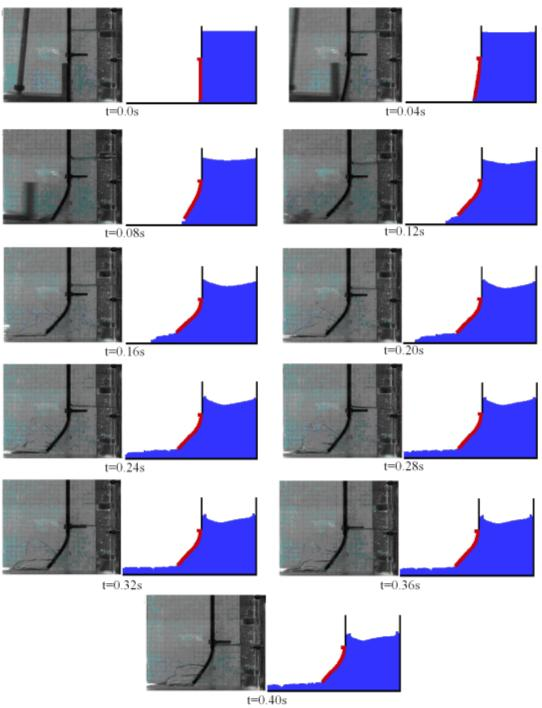
\includegraphics[width=0.9\textwidth]{45-1.png}
\caption{Comparison of experimental results (left) with SPH simulation (right) at different time}\label{fig:45-1}
\end{minipage}
\begin{minipage}[t]{0.05\linewidth}
~
\end{minipage}
\begin{minipage}[t]{0.46\linewidth}
\centering
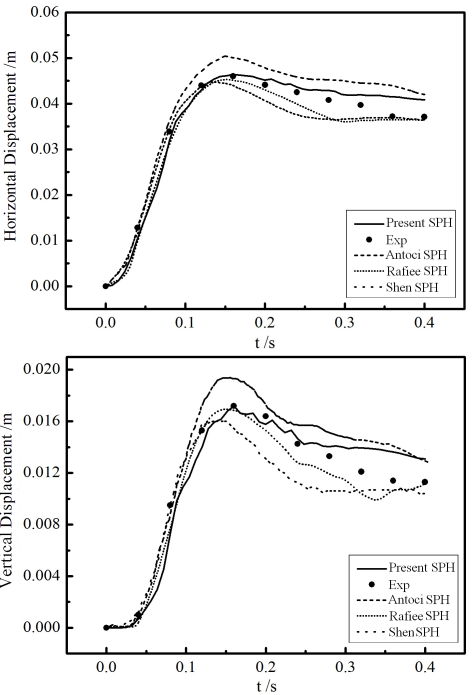
\includegraphics[width=0.8\textwidth]{45-2.png}
\caption{The horizontal and vertical displacement of the free end of the baffle}\label{fig:45-2}
\end{minipage}
\end{figure}


\end{abstract}


%%THE END OF ABSTRACT

\addbib

\end{document}
